\subsection{SOA and Embedded Systems}

Resent topics had a review of available tools and techologies for implementing a
\gls{SOA} system. Most of them are not directly portable to embedded systems.
Related publications \cite{5470528, dguinard-rest-vs-ws} claim that SOA
tools need to be adapted to a constrained hardware by using more lightweight approaches.
Common possibilities are: use of more resource friendly protocols, use of
existing service protocols in a contstrained manner( low request per second
ratio or smaller payload/packet size), use of special constrained protocols,
which are designed specially for interaction between small devices.

This section will describe two possibilities of implementing SOA on an embedded
device, that are based on different research
papers\cite{coap_survey,4221180}.
\nameref{sec:DPWS} section will introduce a
Web Services based device mmcounication framework. \nameref{sec:CoAP} section
will cover RESTful device interactions.
\subsubsection{Devices Profile for Web Services}
\label{sec:DPWS}
The Devices Profile for Web Services (DPWS) was developed to enable secure Web
service capabilities on resource-constrained devices\cite{ws4d_dpws}.
DPWS was mainly developed by Microsoft and some printer device manufacturers.
DPWS allows sending secure messages to and from Web services, discovering a Web service dynamically, describing a Web service, subscribing to, and receiving events from a Web service.


\begin{center}
 \begin{figure}[h]
	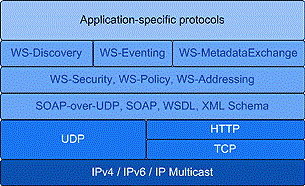
\includegraphics[width=0.5\textwidth]{../images/background/dpws-stack.png}
	\caption{DPWS protocol stack \cite{ws4d_dpws} }
	\label{fig:dpws_protocol_stack}
 \end{figure}
\end{center}


\autoref{fig:dpws_protocol_stack} shows DPWS protocol stack. It is based on  
several Web Services specifications\cite{ws4d_dpws}:
\begin{itemize}
  \item WS-Addressing for advanced endpoint and message addressing
  \item WS-Policy for policy exchange
  \item WS-Security for managing security
  \item WS-Discovery and SOAP-over-UDP for device discovery
  \item WS-Transfer / WS- Metadataexchange for device and service description
  \item WS-Eventing for managing subscriptions for event channels   
\end{itemize}
    
Like Web Services, DPWS uses SOAP, WSDL, XML-Schema. 


DPWS has been ported to several target software
platforms (Linux, Microsoft's Windows and Windows CE,
ExpressLogic's ThreadX and Quadros Systems' Quadros).
It was tested on a processor board comprising a 44-MHz ARM7
TDMI and associated memory (but no cache memory), running
ThreadX. The static memory footprint of the device software including
the OS, the TCP/IP protocol stack and the DPWS software is
less than 500 KB, while the dynamic memory requirements are
below 100 KB.\cite{4221180}.    
Another research \cite{5470528} reports that system disk space
requirements are between 61 and 478 Kbytes. 



\subsubsection{Constrained Application Protocol and Constrained RESTful Environments}
\label{sec:CoAP}

Constrained Application Protocol (CoAP) is a software protocol is
used in very simple electronics devices that allows them to communicate interactively over the Internet.
It is particularly targeted for small low power sensors, switches,
valves and similar components that need to be controlled or supervised remotely, through standard Internet networks.

Lots of applications over the Interent use REST architecture.
   The Constrained RESTful Environments (CoRE) research in IETF organization
   aims to realize the REST architecture in a suitable form for the most
   constrained nodes (e.g.  8-bit microcontrollers with limited RAM and ROM) and
   networks (e.g.  6LoWPAN, IPv6 over Low power Wireless Personal Area
   Networks. RFC4944)~\cite{coap_spec}.

   One of the main goals of CoAP is to design a generic web protocol for
   the special requirements of this constrained environment, especially
   considering energy, building automation and other machine-to-machine
   (M2M) applications.  The purpose of CoAP is to implement a subset of REST
   coupled with HTTP, but optimized for M2M applications.  Although CoAP could
   be used instead of HTTP interfaces because of more compact protocol, it
   also offers features for M2M such as built-in discovery, multicast support and asynchronous message
   exchanges.
      
     CoAP has the following main features:
\begin{itemize}
  \item Constrained web protocol fulfilling M2M requirements.
  \item UDP [RFC0768] binding with optional reliability supporting unicast
      and multicast requests.
  \item Asynchronous message exchanges.
  \item Low header overhead and parsing complexity.
  \item URI and Content-type support.
  \item Simple proxy and caching capabilities.
  \item A stateless HTTP mapping, allowing proxies to be built providing
      access to CoAP resources via HTTP in a uniform way or for HTTP
      simple interfaces to be realized alternatively over CoAP.
  \item Security binding to Datagram Transport Layer Security (DTLS)
      [RFC6347]
\end{itemize}
   
CoAP messages  of two types: requests and responses. 
CoAP uses a short fixed-length binary header (4 bytes) that may be
followed by compact binary options and a payload.
CoAP is by default bound to UDP and optionally to DTLS, providing a high level
of communications security~\cite{wikipedia:coap}.

\subsubsection{Performance issues}

Web services implementations on embedded
devices have quite big overhead. Web service messages are at least 5 times
larger than conventional messages(messages using usual data stuctures, not XML),
messages take at least 2.5 to 2 times longer than conventional
messages, consume more 2 times more energy\cite{5470528}.
Therefore this technology can be only used on hardware with high computational and power
posibilities, not for deeply embedded devices like low-cost microcontrollers for wireless sensors and actuators. 

The second techology, CoAP and RESTful services requires less resources. Its
highly optimized implementation could be executed on a device with 8.5 kB of ROM
and 1.5 kB of RAM \cite{6076698}. It uses Contiki OS and TCP/IP
implementations. This architecture could be a great candidate for  a remote
embedded service.

CoAP was specially designed for constrained devices, while DPWS is a profile
(may be also called a port) of Web services techology to devices, with
complexity of all WS-* technologies. DPWS require more powerful hardware and is
not suitable for the devices where CoAP was designed to run.
